  At a very simple level, neurons are basically computational units that take inputs (\textbf{dendrites}) as electrical inputs (called "spikes") that are channeled to outputs (\textbf{axons}). In our model, our dendrites are like the input features $x_1...x_n$, and the output is the result of our hypothesis function. In this model our $x_0$ input node is sometimes called the "bias unit." It is always equal to 1.

  \begin{figure}[h]
    \centering
    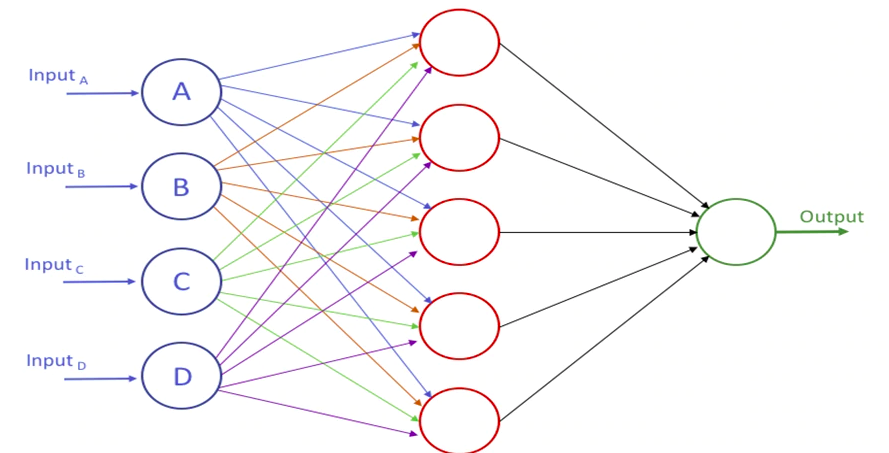
\includegraphics[scale=0.3]{neuralnetwork.png}
  \end{figure}

  Our input nodes (layer 1), also known as the "input layer", go into another node (layer 2), which finally outputs the hypothesis function, known as the "output layer". We can have intermediate layers of nodes between the input and output layers called the "hidden layers."
  \\\\
  These "hidden layer" nodes are called as "activation units". The values for each activation nodes are represented as: \\
  \begin{figure}[h]
    \centering
    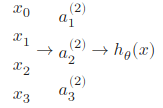
\includegraphics[scale=0.6]{hiddenlayer.png}
  \end{figure}

  \begin{equation}
    a_1^{(2)} = g(\theta_{10}^{(1)}x_0 + \theta_{11}^{(1)}x_1 + \theta_{12}^{(1)}x_2 + \theta_{13}^{(1)}x_3)
  \end{equation}
  \begin{equation}
    a_2^{(2)} = g(\theta_{20}^{(1)}x_0 + \theta_{21}^{(1)}x_1 + \theta_{22}^{(1)}x_2 + \theta_{23}^{(1)}x_3)
  \end{equation}
  \begin{equation}
    a_3^{(2)} = g(\theta_{30}^{(1)}x_0 + \theta_{31}^{(1)}x_1 + \theta_{32}^{(1)}x_2 + \theta_{33}^{(1)}x_3)
  \end{equation}
  \begin{equation}
    h_\theta(x) = a_1^{(3)]} = a_1^{(2)} = g(\theta_{10}^{(2)}x_0 + \theta_{11}^{(2)}x_1 + \theta_{12}^{(2)}x_2 + \theta_{13}^{(2)}x_3)5
  \end{equation}
  \\From these equations, we can conclude that we will get a matrix for each layer to calculate the weight for the second layer.

  \section{Intutions}
    \subsection{OR Function}
      \begin{figure}[h]
        \centering
        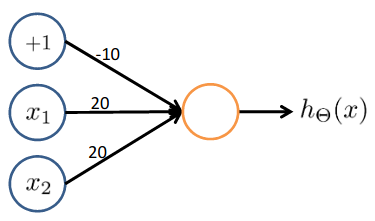
\includegraphics[scale=0.5]{ornet.png}
        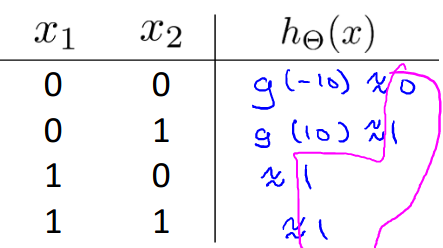
\includegraphics[scale=0.4]{ortable.png}
      \end{figure}

    \subsection{Important Note}
      \begin{figure}[h]
        \centering
        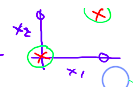
\includegraphics[scale=1]{important-net.png}
      \end{figure}

      For any prediction which involve a straight line as decision boundary, we can represent it with a neural network without any hidden layer but otherwise we'll have to include few hidden layers. An important point to note is that we can represent almost any distribution with cenrain arrangement of neural network.

  \section{Multiclass Classification}
    To classify data into multiple classes, we'll have to define out set of resulting classes as y:
    \begin{figure}[h]
      \centering
      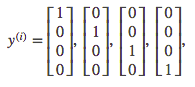
\includegraphics[scale=0.6]{resultnet.png}
    \end{figure}

  \section{Cost Function}
    Let's first define a few variables that we'll need to use:
    
    \begin{itemize}
      \item L = total number of layers in the network
      \item numbers of units (non counting bias unit) in layer 1
      \item K = numbet of output unit/classes
    \end{itemize}

    Cost function for neural networks will be slightly more complicated as it involves few other factors of 'K' and 'L' defined earlier.

    \begin{equation}
      J(\theta) = -\frac{1}{m}\sum_{i=1}^{m}\sum_{k=1}^{K}y_k^{(i)}\log((h_\theta(x^{(i)}))_k) + (1-y_k^{(i)})\log(1-(h_\theta(x^{(i)}))_k) + \frac{\lambda}{2m}\sum_{l=1}^{L-1}\sum_{i=1}^{s_l}\sum_{j=1}^{s_{l+1}} (\theta_{j,i}^{(L)})^2
    \end{equation}

    \textbf{Note:}
    \begin{itemize}
      \item the double sum simply adds up the logistic regression costs calculated for each cell in the output layer.
      \item the triple sum simply adds up the squares of all the individual $\theta$s in the entire network.
      \item the i in the triple sum does not refer to training example i.
    \end{itemize}

  \section{Backpropagation Algorithm}
    Given training set ${(x^(1),y^(1))...(x^(m),y^(m))}$
    \begin{itemize}
      \item Set $\Delta^{(l)}_{i,j} := 0$ for all (l,i,j), (hence you end up having a matrix full of zeros)
    \end{itemize}

    For training example t=1 to m:
    \begin{enumerate}
      \item Set $a^{(1)} := x^{(t)}$
      \item Perform forward propagation to compute $a^{(l)}$ for l = 2,3,...,L

      \textbf{Gradient Computation}

      \item Using $y^{(t)}$, compute $\delta^{(L)} = a^{(L)} - y^{(L)}$
      \item Compute $\delta^{(l)}$
      \item $\Delta^{(L)} := \Delta^{(L)} + \delta^{(l+1)}(a^{(l)})^T$

      \begin{figure}[h]
        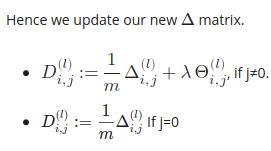
\includegraphics[scale=0.65]{bpupdate.png}
      \end{figure}
    \end{enumerate}

  \section{Gradient Checking}
    Gradient checking will assure that our backpropagation works as intended. We can approximate the derivative of our cost function with:

    \begin{figure}[h]
      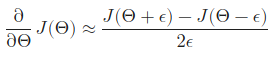
\includegraphics[scale=0.65]{gc.png}
    \end{figure}

    And for multiple features,

    \begin{figure}[h]
      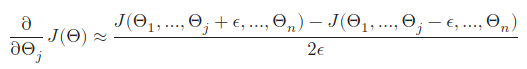
\includegraphics[scale=0.65]{gcmult.png}
    \end{figure}

  \section{Putting it Together}
    First, pick a network architecture; choose the layout of your neural network, including how many hidden units in each layer and how many layers in total you want to have.

    \begin{itemize}
      \item Number of input units = dimension of features $x^{(i)}$
      \item Number of output units = number of classes
      \item Number of hidden units per layer = usually more the better (must balance with cost of computation as it increases with more hidden units)
      \item Defaults: 1 hidden layer. If you have more than 1 hidden layer, then it is recommended that you have the same number of units in every hidden layer.
    \end{itemize}

    \subsubsection{Training a Neural Network}
      \begin{enumerate}
        \item Randomly initialize the weights\footnote[3]{A good choice for $e_init = \frac{\sqrt{6}}{\sqrt{L_in + L_out}}$}
        \item Implement forward propagation to get $h_\theta(x(i))$ for any $x^{(i)}$
        \item Implement the cost function
        \item Implement backpropagation to compute partial derivatives
        \item Use gradient checking to confirm that your backpropagation works. Then disable gradient checking.
        \item Use gradient descent or a built-in optimization function to minimize the cost function with the weights in theta.
      \end{enumerate}
